\documentclass[aspectratio=169]{beamer}
\usepackage{graphicx}
\usepackage{listings}
\usepackage{xcolor}
% SVGs pre-converted to PDF via inkscape

% Custom footline with slide numbers in bottom left
\setbeamertemplate{footline}{
  \hspace{1em}%
  \usebeamercolor[fg]{page number in head/foot}%
  \usebeamerfont{page number in head/foot}%
  \insertframenumber\,/\,\inserttotalframenumber%
  \vskip2pt%
}

\beamertemplatenavigationsymbolsempty

% Code listing style
\lstset{
  basicstyle=\ttfamily\tiny,
  keywordstyle=\color{blue}\bfseries,
  commentstyle=\color{gray}\itshape,
  stringstyle=\color{orange},
  showstringspaces=false,
  breaklines=true,
  frame=single,
  backgroundcolor=\color{gray!10},
  rulecolor=\color{gray!50},
  xleftmargin=2pt,
  xrightmargin=2pt,
  aboveskip=4pt,
  belowskip=4pt,
}

\title{FRIDA Design Review}
\author{Kennedy Caisley}
\date{Wednesday, 28 January 2026}

\begin{document}

\begin{frame}
  \titlepage
\end{frame}

%% ============================================================
%% ADC Target Specifications
%% ============================================================
\begin{frame}
  \frametitle{ADC Target Specifications}
  \begin{center}
    \small
    \begin{tabular}{l|ccccc}
      \hline
      \textbf{Parameter} & \textbf{DCD v1} & \textbf{CoRDIA} & \textbf{M} & \textbf{H} & \textbf{F (target)} \\
      \hline
      Resolution          & 8-bit       & 10-bit     & 8-bit      & 10-bit      & 12-bit      \\
      ENOB                & 8.3         & 8.8        & 8.0        & 9.5?        & 11.0?       \\
      Conversion rate     & 6.25 MHz    & 2.5 MHz    & 4.5 MHz    & 10 MHz      & 10 MHz      \\
      ADC dimensions      & 40$\times$55 $\mu$m & 80$\times$330 $\mu$m & 60$\times$800 $\mu$m & 15$\times$100 $\mu$m & 50$\times$50 $\mu$m \\
      ADC area            & 0.002 mm$^2$ & 0.026 mm$^2$ & 0.048 mm$^2$ & 0.0015 mm$^2$ & 0.0025 mm$^2$ \\
      Power per ADC       & 960 $\mu$W  & 30 $\mu$W  & 700 $\mu$W & 100 $\mu$W  & 200 $\mu$W? \\
      FOM$_{\mathrm{csa}}$ (Hz/$\mu$m$^2$) & 3125 & 95 & 105 & 5000 & 5000 \\
      FOM$_{\mathrm{wal}}$ (fJ/conv-step) & 487 & 26 & 608 & 14 & 10 \\
      \hline
    \end{tabular}
  \end{center}
  \vspace{0.5em}
  \begin{itemize}
    \item \textbf{F} = FRIDA target: 12-bit, 10 MHz, 50$\times$50 $\mu$m footprint
    \item FOM$_{\mathrm{csa}}$ = conversion rate / area; FOM$_{\mathrm{wal}}$ = energy per conversion step
  \end{itemize}
\end{frame}

%% ============================================================
%% Floorplan Overview (ASCII)
%% ============================================================
\begin{frame}[fragile]
  \frametitle{Sketch of ADC Floorplan}
  \begin{center}
  \begin{lstlisting}[basicstyle=\ttfamily\fontsize{4}{5}\selectfont,frame=none,backgroundcolor=\color{white}]
            Logic and Macro Placement (FEOL-M3)           Power Domain Placement (M3-M4)              Capacitor DAC Arrays (M5-M6)
            -----------------------------------           ------------------------------              ----------------------------

     +-    +----------------------------------+        +----------------------------------+        +---------------+  +---------------+
2 Tr |     |         Cap Drivers (diff)       |        |         vdd_dac & vss_dac        |        |    (pins)     |  |    (pins)     |
     +-    +----------------------------------+        +----------------------------------+        |               |  |               |
     +-    +---+ +------++------++------+ +---+             +------------------------+             |               |  |               |
     |     |   | |      ||      ||      | |   |             |                        |             |               |  |               |
5 Tr |     |   | | SW N || Comp || SW P | |   |             |     vdd_a & vss_a      |             |               |  |               |
     |     |   | |      ||      ||      | |   |             |                        |             |               |  |               |
     +-    |   | +------++------++------+ |   |             +------------------------+             |               |  |               |
     +-    |   +---------------------------   |        +----------------------------------+        |               |  |               |
     |     |                                  |        |                                  |        |               |  |               |
     |     |                                  |        |                                  |        |               |  |               |
     |     |                                  |        |                                  |        |               |  |               |
     |     |                                  |        |                                  |        |  P Cap Array  |  |  N Cap Array  |
     |     |                                  |        |                                  |        |               |  |               |
8 Tr |     |        SA Logic, Clk Gate,       |        |          vdd_d & vss_d           |        |               |  |               |
     |     |           & Samp Driver          |        |                                  |        |               |  |               |
     |     |                                  |        |                                  |        |               |  |               |
     |     |                                  |        |                                  |        |               |  |               |
     |     |                                  |        |                                  |        |               |  |               |
     |     |                                  |        |                                  |        |               |  |               |
     +-    +----------------------------------+        +----------------------------------+        |               |  |               |
     +-    +----------------------------------+        +----------------------------------+        |               |  |               |
2 Tr |     |        Cap Drivers (main)        |        |        vref_p  & vref_n          |        |    (pins)     |  |    (pins)     |
     +-    +----------------------------------+        +----------------------------------+        +---------------+  +---------------+
  \end{lstlisting}
  \end{center}
\end{frame}

%% ============================================================
%% Unit Fringe Capacitor
%% ============================================================
\begin{frame}
  \frametitle{Unit Fringe Capacitor}
  \begin{columns}
    \begin{column}{0.5\textwidth}
      1 layer: $0.31~\mathrm{fF}/\mu\mathrm{m}^2$ \\
      2 layers: $0.62~\mathrm{fF}/\mu\mathrm{m}^2$ \\
      3 layers: $0.93~\mathrm{fF}/\mu\mathrm{m}^2$ \\[1em]
      Matching coefficient: $\sigma(\Delta C/C) = 0.85\% \times \sqrt{C~[\mathrm{fF}]}$
      \vspace{2em}
      \begin{center}
        \includegraphics[width=\linewidth,height=0.4\textheight,keepaspectratio]{images/cdac_unit_cell_3d.png}
      \end{center}
    \end{column}
    \begin{column}{0.5\textwidth}
      \begin{center}
        \includegraphics[width=\linewidth,height=0.8\textheight,keepaspectratio]{images/cdac_unit_cell.png}
      \end{center}
    \end{column}
  \end{columns}
\end{frame}

%% ============================================================
%% CDAC Array Overview
%% ============================================================
\begin{frame}
  \frametitle{CDAC Array Overview}
  \begin{columns}
    \begin{column}{0.5\textwidth}
      \[
        \text{Total Area} = 1940~\mu\mathrm{m}^2
      \]
      \[
        C_\mathrm{tot} = 1.4~\mathrm{pF}
      \]
      \begin{center}
        \includegraphics[width=\linewidth,height=0.5\textheight,keepaspectratio]{images/cdac_array_3d.png}
      \end{center}
    \end{column}
    \begin{column}{0.5\textwidth}
      \begin{center}
        \includegraphics[width=\linewidth,height=0.85\textheight,keepaspectratio]{images/cdac_array.png}
      \end{center}
    \end{column}
  \end{columns}
\end{frame}

%% ============================================================
%% ADC Digital Netlist
%% ============================================================
\begin{frame}
  \frametitle{ADC Digital Block Netlist}
  \begin{columns}
    \begin{column}{0.35\textwidth}
      \begin{itemize}
        \item \textbf{salogic}: SAR sequencing FSM
        \item \textbf{clkgate}: Clock gating for power
        \item \textbf{sampdriver\_p/n}: Sampling switch drivers
        \item Symmetric P/N halves for differential operation
        \item salogic and clkgate shared between halves
      \end{itemize}
    \end{column}
    \begin{column}{0.65\textwidth}
      \begin{center}
        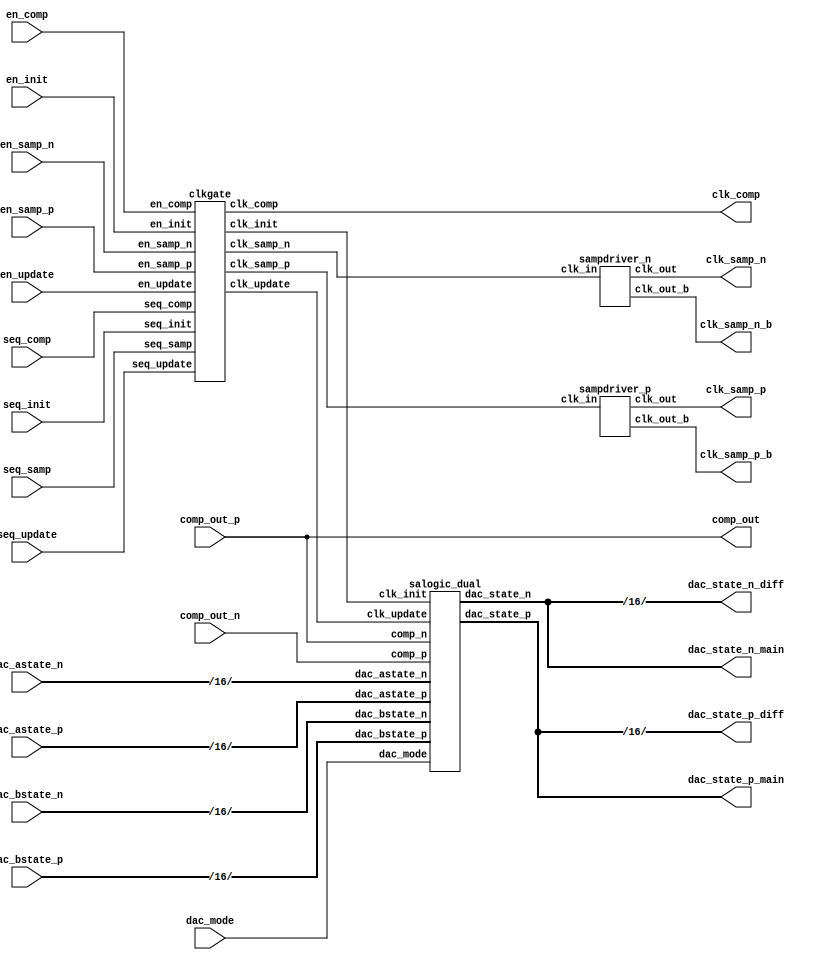
\includegraphics[width=\linewidth,height=0.85\textheight,keepaspectratio]{images/adc_digital_netlistsvg.pdf}
      \end{center}
    \end{column}
  \end{columns}
\end{frame}

%% ============================================================
%% OpenROAD Flow Scripts Overview
%% ============================================================
\begin{frame}
  \frametitle{OpenROAD Flow Scripts (ORFS)}
  \begin{columns}
    \begin{column}{0.5\textwidth}
      \begin{itemize}
        \item \textbf{Yosys}: RTL synthesis
          \begin{itemize}
            \item Verilog parsing and elaboration
            \item Logic optimization (ABC)
            \item Technology mapping to standard cells
          \end{itemize}
        \item \textbf{OpenROAD}: Physical design
          \begin{itemize}
            \item Floorplanning and PDN
            \item Placement (global + detailed)
            \item Clock tree synthesis
            \item Routing (global + detailed)
            \item Timing analysis (OpenSTA)
          \end{itemize}
        \item \textbf{KLayout}: Final verification
          \begin{itemize}
            \item DRC and LVS checks
            \item GDS export
          \end{itemize}
      \end{itemize}
    \end{column}
    \begin{column}{0.5\textwidth}
      \begin{center}
        \includegraphics[width=\linewidth,height=0.85\textheight,keepaspectratio]{images/orfs.png}
      \end{center}
    \end{column}
  \end{columns}
\end{frame}

%% ============================================================
%% Yosys: Step 1 - Synthesis
%% ============================================================
\begin{frame}[fragile]
  \frametitle{Yosys: Step 1 - RTL Synthesis}
  \begin{columns}
    \begin{column}{0.5\textwidth}
      \textbf{Input Files}
      \begin{itemize}
        \item adc\_digital.v (top module)
        \item clkgate.v, salogic.v, sampdriver.v
        \item cells\_tsmc65.v (cell wrappers)
      \end{itemize}
      \vspace{1em}
      \textbf{Synthesis Statistics}
      \begin{itemize}
        \item Total cells: 350
        \item Total area: 893.88 $\mu$m$^2$
        \item Sequential elements: 49.6\% of area
        \item 48 flip-flops (DFQD1, EDFD2)
        \item 5 clock gates (CKLNQD1LVT)
      \end{itemize}
    \end{column}
    \begin{column}{0.5\textwidth}
      \textbf{Technology Mapping (ABC)}
      \begin{lstlisting}[basicstyle=\ttfamily\scriptsize]
Module         Cells    Area
---------------------------------
adc_digital       38    54.36
  clkgate          6    33.48
  salogic        302   798.84
  sampdriver       2     3.60
---------------------------------
Total            350   893.88
      \end{lstlisting}
      \vspace{0.5em}
      \textbf{Key Cell Types}
      \begin{lstlisting}[basicstyle=\ttfamily\scriptsize]
EDFD2LVT (edge DFF)     32   334.08
DFQD1LVT (DFF)          16   109.44
NR2D0LVT (NOR2)         93   133.92
BUFFD0LVT (buffer)      69    99.36
CKLNQD1LVT (clkgate)     5    32.40
      \end{lstlisting}
    \end{column}
  \end{columns}
\end{frame}

%% ============================================================
%% OpenROAD Step 2.1 Floorplan
%% ============================================================
\begin{frame}[fragile]
  \frametitle{OpenROAD Step 2.1: Floorplan}
  \begin{columns}
    \begin{column}{0.45\textwidth}
      \begin{center}
        \includegraphics[width=\linewidth,height=0.85\textheight,keepaspectratio]{images/2_0_floorplan.png}
      \end{center}
    \end{column}
    \begin{column}{0.55\textwidth}
      \begin{itemize}
        \item Die and core area: 60$\mu$m $\times$ 49$\mu$m
        \item Row height: 2.8$\mu$m (17 rows)
        \item Blockages reserve space for analog macros
        \item Custom I/O pin placement for DAC interface
      \end{itemize}
      \vspace{1em}
      \textbf{config.mk}
      \begin{lstlisting}[language=make]
export DIE_AREA = 0 0 60 49
export CORE_AREA = 0 0 60 49
export CREATE_BLOCKAGES = .../create_blockages.tcl
      \end{lstlisting}
      \textbf{create\_blockages.tcl}
      \begin{lstlisting}[language=tcl]
# Reserve area for comparator
create_blockage -region {17.5 27.0 42.5 49}
# Reserve areas for sampling switches
create_blockage -region {12.5 42.6 21 49}
create_blockage -region {39 42.6 47.5 49}
      \end{lstlisting}
    \end{column}
  \end{columns}
\end{frame}

%% ============================================================
%% OpenROAD Step 2.2 Floorplan with PDN
%% ============================================================
\begin{frame}[fragile]
  \frametitle{OpenROAD Step 2.2: Power Distribution Network}
  \begin{columns}
    \begin{column}{0.45\textwidth}
      \begin{center}
        \includegraphics[width=\linewidth,height=0.85\textheight,keepaspectratio]{images/2_4_floorplan_pdn.png}
      \end{center}
    \end{column}
    \begin{column}{0.55\textwidth}
      \begin{itemize}
        \item M4 vertical stripes at edges for vdd\_d/vss\_d
        \item M1 horizontal stripes follow standard cell rows
        \item M1-M4 connections for power delivery
      \end{itemize}
      \vspace{1em}
      \textbf{pdn.tcl}
      \begin{lstlisting}[language=tcl]
add_global_connection -net {vdd_d} \
  -inst_pattern {.*} -pin_pattern VDD -power
add_global_connection -net {vss_d} \
  -inst_pattern {.*} -pin_pattern VSS -ground

define_pdn_grid -name "Core" -pins {M4}

add_pdn_stripe -grid "Core" -layer M4 \
  -width 0.4 -offset 1.3 -nets {vdd_d}
add_pdn_stripe -grid "Core" -layer M4 \
  -width 0.4 -offset 2.1 -nets {vss_d}

add_pdn_stripe -grid "Core" -layer M1 \
  -followpins -width 0.33
add_pdn_connect -grid "Core" -layers {M1 M4}
      \end{lstlisting}
    \end{column}
  \end{columns}
\end{frame}

%% ============================================================
%% OpenROAD Step 3.1 Global Placement (Skip IO)
%% ============================================================
\begin{frame}[fragile]
  \frametitle{OpenROAD Step 3.1: Global Placement (Skip I/O)}
  \begin{columns}
    \begin{column}{0.45\textwidth}
      \begin{center}
        \includegraphics[width=\linewidth,height=0.85\textheight,keepaspectratio]{images/3_1_place_gp_skip_io.png}
      \end{center}
    \end{column}
    \begin{column}{0.55\textwidth}
      \begin{itemize}
        \item Initial cell spreading before I/O placement
        \item Routability-driven placement disabled (OpenROAD bug)
        \item 50\% target placement density
      \end{itemize}
      \vspace{1em}
      \textbf{config.mk}
      \begin{lstlisting}[language=make]
# Disable routability-driven placement
# due to OpenROAD crash in cutFillerCells()
export GPL_ROUTABILITY_DRIVEN = 0

# Standard cell placement density
export PLACE_DENSITY = 0.50

# I/O pin layers
export IO_PLACER_H = M3
export IO_PLACER_V = M2
      \end{lstlisting}
    \end{column}
  \end{columns}
\end{frame}

%% ============================================================
%% OpenROAD Step 3.2 Global Placement
%% ============================================================
\begin{frame}[fragile]
  \frametitle{OpenROAD Step 3.2: Global Placement}
  \begin{columns}
    \begin{column}{0.45\textwidth}
      \begin{center}
        \includegraphics[width=\linewidth,height=0.85\textheight,keepaspectratio]{images/3_3_place_gp.png}
      \end{center}
    \end{column}
    \begin{column}{0.55\textwidth}
      \begin{itemize}
        \item I/O pins now placed on die boundary
        \item DAC pins on left/right edges (M3), 2.8$\mu$m spacing
        \item Control signals on bottom (M2)
      \end{itemize}
      \vspace{1em}
      \textbf{io.tcl}
      \begin{lstlisting}[language=tcl]
# Left side - DAC astate positive pins
place_pin -pin_name dac_astate_p[0] \
  -layer M3 -location {0.0 5.6} \
  -force_to_die_boundary

# Right side - DAC astate negative pins
place_pin -pin_name dac_astate_n[0] \
  -layer M3 -location {60.0 5.6} \
  -force_to_die_boundary

# Bottom - Control signals
place_pin -pin_name seq_update \
  -layer M2 -location {32.9 0.0} \
  -force_to_die_boundary
      \end{lstlisting}
    \end{column}
  \end{columns}
\end{frame}

%% ============================================================
%% OpenROAD Step 3.3 Detailed Placement
%% ============================================================
\begin{frame}[fragile]
  \frametitle{OpenROAD Step 3.3: Detailed Placement}
  \begin{columns}
    \begin{column}{0.45\textwidth}
      \begin{center}
        \includegraphics[width=\linewidth,height=0.85\textheight,keepaspectratio]{images/3_5_place_dp.png}
      \end{center}
    \end{column}
    \begin{column}{0.55\textwidth}
      \begin{itemize}
        \item Cells snapped to placement grid
        \item Critical buffers protected from removal
        \item Clock gate and sample driver cells preserved
      \end{itemize}
      \vspace{1em}
      \textbf{dont\_touch.tcl}
      \begin{lstlisting}[language=tcl]
# Protect sampdriver instances
set sampdriver_instances [get_cells -quiet \
  -filter "full_name =~ sampdriver_*"]
foreach inst $sampdriver_instances {
    set_dont_touch $inst
}

# Protect clkgate cells (TSMC65 CKLNQD1LVT)
set clkgate_cells [get_cells -quiet \
  -filter "ref_name == CKLNQD1LVT"]
foreach inst $clkgate_cells {
    set_dont_touch $inst
}
      \end{lstlisting}
    \end{column}
  \end{columns}
\end{frame}

%% ============================================================
%% OpenROAD Step 4.1 Clock Tree Synthesis
%% ============================================================
\begin{frame}[fragile]
  \frametitle{OpenROAD Step 4.1: Clock Tree Synthesis}
  \begin{columns}
    \begin{column}{0.45\textwidth}
      \begin{center}
        \includegraphics[width=\linewidth,height=0.85\textheight,keepaspectratio]{images/4_1_cts.png}
      \end{center}
    \end{column}
    \begin{column}{0.55\textwidth}
      \begin{itemize}
        \item System clock: 10 MHz (100ns period)
        \item Samp/comp clock: 200 MHz (5ns period)
        \item 50ps clock uncertainty
        \item Balanced tree for minimal skew
      \end{itemize}
      \vspace{1em}
      \textbf{constraint.sdc}
      \begin{lstlisting}[language=tcl]
current_design adc_digital

# Create clock for sequencing (200 MHz)
create_clock -name seq_update \
  -period 5 [get_ports seq_update]

# Set clock uncertainties
set_clock_uncertainty 0.05 [all_clocks]
      \end{lstlisting}
    \end{column}
  \end{columns}
\end{frame}

%% ============================================================
%% OpenROAD Step 4.1 Clock Tree Views
%% ============================================================
\begin{frame}
  \frametitle{OpenROAD Step 4.1: Clock Tree Views}
  \begin{columns}
    \begin{column}{0.5\textwidth}
      \begin{center}
        \includegraphics[width=0.9\linewidth,height=0.55\textheight,keepaspectratio]{images/4_1_cts_alt.png}
      \end{center}
    \end{column}
    \begin{column}{0.5\textwidth}
      \begin{center}
        \includegraphics[width=0.9\linewidth,height=0.45\textheight,keepaspectratio]{images/4_1_treeview.png}
      \end{center}
    \end{column}
  \end{columns}
  \vspace{0.5em}
  \begin{center}
    \small
    \textbf{CTS Results:} $f_{\mathrm{max}}$ = 1760 MHz \quad|\quad
    Worst slack = 4.43 ns \quad|\quad
    Setup skew = 0.07 ns \quad|\quad
    Power = 182 $\mu$W
  \end{center}
\end{frame}

%% ============================================================
%% OpenROAD Step 5.1 Global Routing
%% ============================================================
\begin{frame}[fragile]
  \frametitle{OpenROAD Step 5.1: Global Routing}
  \begin{columns}
    \begin{column}{0.45\textwidth}
      \begin{center}
        \includegraphics[width=\linewidth,height=0.85\textheight,keepaspectratio]{images/5_1_routeguides_global.png}
      \end{center}
    \end{column}
    \begin{column}{0.55\textwidth}
      \begin{itemize}
        \item Route guides shown for global routing
        \item M2-M3 routing layers only
        \item Routing obstructions for analog areas
      \end{itemize}
      \vspace{1em}
      \textbf{config.mk}
      \begin{lstlisting}[language=make]
export MIN_ROUTING_LAYER = M2
export MAX_ROUTING_LAYER = M3
export PRE_GLOBAL_ROUTE_TCL = \
  .../routing_blockages.tcl
      \end{lstlisting}
      \textbf{routing\_blockages.tcl}
      \begin{lstlisting}[language=tcl]
# Create obstructions on M1-M4 for analog
odb::dbObstruction_create $block $layer_M1 \
  $comp_llx $comp_lly $comp_urx $comp_ury
odb::dbObstruction_create $block $layer_M2 \
  $comp_llx $comp_lly $comp_urx $comp_ury
      \end{lstlisting}
    \end{column}
  \end{columns}
\end{frame}

%% ============================================================
%% OpenROAD Step 5.2 Detailed Routing
%% ============================================================
\begin{frame}[fragile]
  \frametitle{OpenROAD Step 5.2: Detailed Routing}
  \begin{columns}
    \begin{column}{0.45\textwidth}
      \begin{center}
        \includegraphics[width=\linewidth,height=0.85\textheight,keepaspectratio]{images/5_2_route.png}
      \end{center}
    \end{column}
    \begin{column}{0.55\textwidth}
      \begin{itemize}
        \item Final metal routing on M2/M3
        \item All signals routed to I/O pins
        \item DRC-clean routing around blockages
      \end{itemize}
      \vspace{1em}
      \textbf{config.mk}
      \begin{lstlisting}[language=make]
# Based on TSMC65LP metal stack
# from tcbn65lp_9lmT2.lef
export MIN_ROUTING_LAYER = M2
export MAX_ROUTING_LAYER = M3
      \end{lstlisting}
    \end{column}
  \end{columns}
\end{frame}

%% ============================================================
%% OpenROAD Step 5.3 Fill Cells
%% ============================================================
\begin{frame}[fragile]
  \frametitle{OpenROAD Step 5.3: Fill Cells}
  \begin{columns}
    \begin{column}{0.45\textwidth}
      \begin{center}
        \includegraphics[width=\linewidth,height=0.85\textheight,keepaspectratio]{images/5_3_fillcell.png}
      \end{center}
    \end{column}
    \begin{column}{0.55\textwidth}
      \begin{itemize}
        \item Decap fill cells added (FEOL)
        \item Metal fill disabled (BEOL)
        \item Fills gaps in standard cell rows
      \end{itemize}
      \vspace{1em}
      \textbf{config.mk}
      \begin{lstlisting}[language=make]
# Only disables metal fill
# FILL_CELLS in routing step still
# adds FEOL decap fill cells
export USE_FILL = 0
      \end{lstlisting}
    \end{column}
  \end{columns}
\end{frame}

%% ============================================================
%% OpenROAD Step 6.1 Heat Maps
%% ============================================================
\begin{frame}
  \frametitle{OpenROAD Step 6.1: Heat Maps}
  \begin{columns}
    \begin{column}{0.45\textwidth}
      \begin{center}
        \includegraphics[width=\linewidth,height=0.85\textheight,keepaspectratio]{images/6_2_thermal.png}
      \end{center}
    \end{column}
    \begin{column}{0.55\textwidth}
      \begin{center}
        \includegraphics[width=\linewidth,height=0.5\textheight,keepaspectratio]{images/power.png}
      \end{center}
      \vspace{0.5em}
      \begin{itemize}
        \item Spatial visualizations for IR drop, thermal dissipation, placement density, pin density, and power consumption are available
      \end{itemize}
    \end{column}
  \end{columns}
\end{frame}

%% ============================================================
%% OpenROAD GUI
%% ============================================================
\begin{frame}
  \frametitle{OpenROAD GUI}
  \begin{itemize}
    \item Interactive GUI, net tracing, hierarchical cell grouping, timing reports, DRC viewer, heatmaps
  \end{itemize}
  \begin{center}
    \includegraphics[width=\linewidth,height=0.78\textheight,keepaspectratio]{images/openroad_gui.png}
  \end{center}
\end{frame}

%% ============================================================
%% ADC Top Assembly
%% ============================================================
\begin{frame}
  \frametitle{ADC Top-Level Assembly}
  \begin{center}
    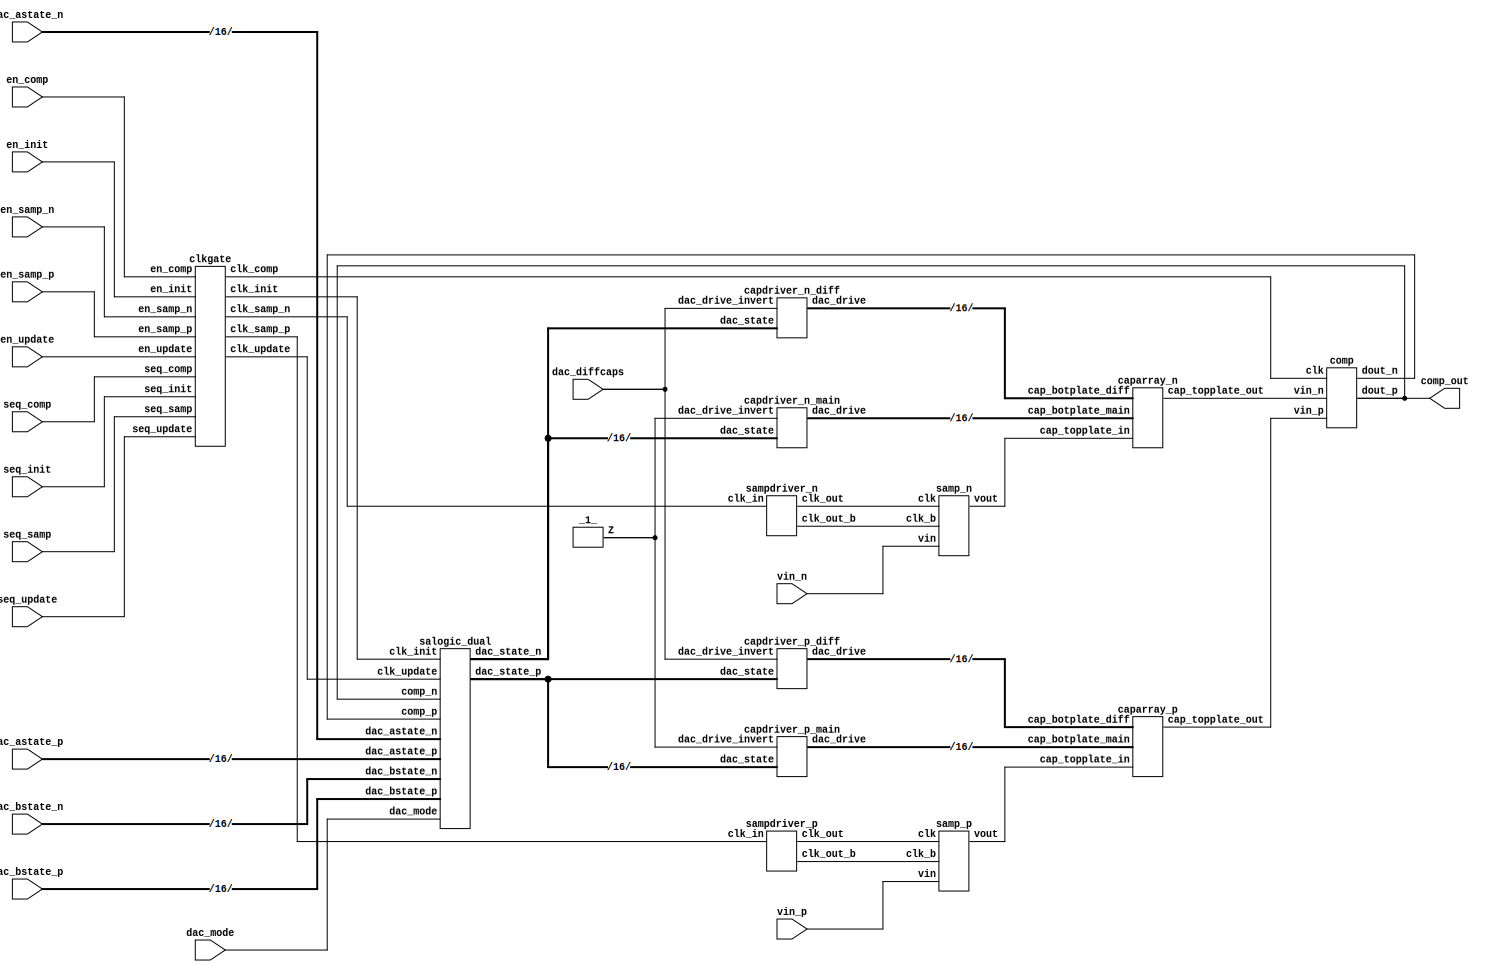
\includegraphics[width=\linewidth,height=0.75\textheight,keepaspectratio]{images/adc_top_netlistsvg.pdf}
  \end{center}
  \begin{itemize}
    \item ADC assembled using hierarchical Verilog as well, with protected routing for sensitive analog nets
  \end{itemize}
\end{frame}

%% ============================================================
%% ADC Level Integration
%% ============================================================
\begin{frame}
  \frametitle{ADC Level Integration}
  \begin{center}
    \includegraphics[width=\linewidth,height=0.85\textheight,keepaspectratio]{images/frida_status.pdf}
  \end{center}
\end{frame}

\end{document}
